\documentclass[xcolor=dvipsnames]{beamer}

\usepackage{setspace}
\usepackage{beamerthemesplit}
\usepackage{graphicx}
\usepackage{epstopdf}
\usepackage[english]{babel}
\usepackage[latin1]{inputenc}
\usepackage{times}
\usepackage[T1]{fontenc}
\usepackage{color}
\usepackage{colortbl}
\usepackage[noend]{algorithm,algpseudocode}
\usepackage{multimedia,xmpmulti}
\usepackage{multirow,multicol}
\usepackage[absolute,overlay]{textpos}
\usepackage{multimedia,xmpmulti}
\usepackage{tabularx,multicol}
\usepackage{url}
\usepackage{ulem}
\usepackage{stackengine}
\stackMath

%\input{tensor_header}

%% Tikz - For making pretty pictures
\usepackage{tikz}
\usetikzlibrary{3d}
\usetikzlibrary{patterns}
\usetikzlibrary{calc}
\usetikzlibrary{arrows}

\usepackage{pgfplots}
\usepackage{pgfplotstable}
\usepackage{etoolbox}
%\pgfplotsset{compat=1.12}
\usetikzlibrary{decorations.pathreplacing}
\makeatletter
\newcommand{\gettikzxy}[3]{%
\tikz@scan@one@point\pgfutil@firstofone#1\relax
\edef#2{\the\pgf@x}%
\edef#3{\the\pgf@y}%
}
\makeatother
\newcommand{\datafile}{}

\algrenewcommand{\algorithmiccomment}[1]{\textit{$\%$ #1}}
\newcommand{\lt}{\left}
\newcommand{\rt}{\right}
\newcommand{\ra}{\rightarrow}
\newcommand{\dis}{\displaystyle}
\newcommand{\bc}[3]{\left\langle#1, #2, #3\right\rangle}
\DeclareMathOperator*{\argmin}{arg\,/min}
\newcommand{\ignore}[1]{}
\newtheorem{thm}{Theorem}
\newtheorem{lem}[thm]{Lemma}
\definecolor{bgblue}{rgb}{0.8,0.85,1}
\definecolor{bggreen}{rgb}{0.8,1,0.8}
\definecolor{bgred}{rgb}{1,0.85,0.8}
\definecolor{Blue}{rgb}{.08,0,.7}
\setbeamercolor{greentextbox}{fg=black,bg=bggreen}

\definecolor{wfugold}{rgb}{0.6196078,0.494117647,0.21960784}
\newcommand{\red}[1]{\textcolor{red}{#1}}
\newcommand{\blue}[1]{\textcolor{blue}{#1}}
\newcommand{\multiplycolor}{red}
\newcommand{\zero}{}
\newcommand{\cred}[1]{\textcolor{red}{#1}}
\newcommand{\cblue}[1]{\textcolor{blue}{#1}}
\newcommand{\cgold}[1]{\textcolor{wfugold}{#1}}

\newcommand{\UVW}{\llbracket \M U, \M V, \M W \rrbracket}
\newcommand{\plusequals}{\mathrel{+}=}
\algdef{SE}[FORDOTS]{ForDots}{EndForDots}{$\ddots$}{}


\newlength\matfield
\newlength\tmplength
\def\matscale{1.}
\newcommand\dimbox[3]{%
\setlength\matfield{\matscale\baselineskip}%
\setbox0=\hbox{\vphantom{X}\smash{#3}}%
\setlength{\tmplength}{#1\matfield-\ht0-\dp0}%
\fboxrule=1pt\fboxsep=-\fboxrule\relax%
\fbox{\makebox[#2\matfield]{\addstackgap[.5\tmplength]{\box0}}}%
}
\newcommand\raiserows[2]{%
\setlength\matfield{\matscale\baselineskip}%
\raisebox{#1\matfield}{#2}%
}
\newcommand\matbox[5]{
\stackunder{\dimbox{#1}{#2}{$#5$}}{\scriptstyle(#3\times #4)}%
}

\graphicspath{{fig/}}

\mode<presentation>

\usetheme{Warsaw}
\usecolortheme[named=wfugold]{structure}
%Madrid
%\usecolortheme{dolphin}
%\useinnertheme{rounded}
%\usefonttheme{serif}
\setbeamertemplate{navigation symbols}{} % gets rid of navigation bars
\setbeamertemplate{footline}
{
\hbox{
\begin{beamercolorbox}[wd=.33\paperwidth,ht=2.25ex,dp=1ex,left]{author in head/foot}%
\usebeamerfont{author in head/foot}
Manning
\end{beamercolorbox}%
\begin{beamercolorbox}[wd=.34\paperwidth,ht=2.25ex,dp=1ex,center]{title in head/foot}%
\usebeamerfont{title in head/foot}

\end{beamercolorbox}%
\begin{beamercolorbox}[wd=.33\paperwidth,ht=2.25ex,dp=1ex,right]{date in head/foot}%
\usebeamerfont{date in head/foot}
\insertframenumber{} \hspace*{2ex}
\end{beamercolorbox}}%
}

\definecolor{christ}{HTML}{ff0012}
\definecolor{mas}{HTML}{00b32c}

\pgfplotsset{compat=1.16}

\begin{document}

\title{Rank-2 Nonnegative Matrix Factorization (R2NMF)}
\author[Manning]{\textbf{Lawton Manning}, Grey Ballard, et. al.}
\institute{
\includegraphics[scale=.15]{wfulogo}}
\date{December 5, 2019}
\begin{frame}[label=title,plain]
\maketitle
\end{frame}
\addtocounter{framenumber}{-1}

\begin{frame}{Introduction to NMF}
\begin{itemize}
\item Nonnegative Matrix Factorization
\item given $A$, compute $W$ and $H$ such that
\begin{itemize}
\item $A \approx WH^T$
\end{itemize}
\item NP-hard optimization problem
\item comparable to K-means clustering in Data Mining
\end{itemize}
\end{frame}

\begin{frame}{General NMF}
\begin{center}
$
\renewcommand\matscale{1}
\matbox{10}{5}{m}{n}{\mathrm{A}} \approx
\matbox{10}{1}{m}{k}{W}
\raiserows{4.5}{\matbox{1}{5}{k}{n}{H^T}}
$
\end{center}
\begin{itemize}
\item Choose a $k$ such that $W$ and $H$ are both tall and skinny matrices.
\item each of the $k$ columns in $W$ and $H$ represent important features shared among rows and columns of $A$
\end{itemize}
\end{frame}

\begin{frame}{Hierarchical Document Clustering}
\begin{itemize}
\item \textbf{idea}: repeatedly use a $k=2$ NMF to split a set of documents (cols) into two clusters based on their words (rows)
\item \textbf{algorithm}: at each level, use the info in $W$ and $H$ to split $A$ into two clusters and repeat the algorithm on the sub-matrices
\item \textbf{result}: produces binary tree of hierarchical clusters of the documents by important words shared between documents in a cluster
\end{itemize}
\end{frame}


\begin{frame}{Hierarchical Document Clustering cont.}
\begin{tikzpicture}[scale=0.8]
\fill[christ] (0,0) rectangle (0.5,4);
\fill[mas] (0.5,0) rectangle (1.5,4);
\fill[christ] (1.5,0) rectangle (3,4);
\fill[mas] (3,0) rectangle (4,4);

\draw[thick] (0.25,0) parabola (1.5,-0.5);
\draw[thick] (2.25,0) parabola (1.5,-0.5);

\draw[thick] (1,4) parabola (1.75,4.5);
\draw[thick] (3.5,4) parabola (1.75,4.5);

\fill[christ] (8,-2.2) rectangle (10,1.8);
\fill[mas] (8,6.2) rectangle (10,2.2);

\draw[thick,->] (1.5,-0.5) .. controls (1.5,-2) and (5,0) .. (8,-0.2);
\draw[thick,->] (1.75,4.5) .. controls (4,6) and (5,4) .. (8, 4.2);

\end{tikzpicture}

\begin{itemize}
\item We can split $A$ into $A_1$ and $A_2$ by using columns $w_1$ and $w_2$
\end{itemize}
\end{frame}

\begin{frame}{NMF Algorithm}
$
\renewcommand\matscale{1}
\matbox{2.5}{4}{k}{m}{W^T}\times 
\matbox{4}{2.5}{m}{k}{W}
=
\matbox{2.5}{2.5}{k}{k}{W^TW}
$
$
\renewcommand\matscale{1}
\matbox{2.5}{4}{k}{m}{W^T}\times
\matbox{4}{6}{m}{n}{A}
=
\matbox{2.5}{6}{k}{n}{W^TA}
$
\begin{itemize}
\item update $W$ and $H$ alternatively by solving for one with the other fixed
\item \textbf{W:} compute $H^TH$ and $(AH)^T$
\item \textbf{H:} compute $W^TW$ and $W^TA$
\end{itemize}
\end{frame}

\begin{frame}{R2NMF Algorithm}
\begin{center}
\begin{tikzpicture}[scale=0.29]

%W1
\draw (0,0) rectangle (1.25,18) node[midway] {\tiny $w_1$};
%W2
\draw (1.25,0) rectangle (2.5,18) node[midway] {\tiny $w_2$};

%H1
\draw (3,19.75) rectangle (15,21) node[midway] {\tiny $h_1^T$};
%H2
\draw (3,18.5) rectangle (15,19.75) node[midway] {\tiny $h_2^T$};

%A
\draw (3,0) rectangle (15,18) node[midway] {$A$};

\end{tikzpicture}
\end{center}

\begin{itemize}
\item with $k=2$, we can treat the columns of $W$ and $H$ as vectors and use \textbf{matrix-vector} multiply to solve for them
\end{itemize}
\end{frame}

\begin{frame}{Data Distribution for MPI}
\begin{center}
\begin{tikzpicture}[scale=0.29]

%W
\draw (1.875,0) node[below] {$W$};
\draw (1.25,0) rectangle (2.5,18);
\fill[red] (1.25,18) rectangle (2.5,15);
\fill[orange] (1.25,15) rectangle (2.5,12);
\fill[yellow] (1.25,12) rectangle (2.5,9);
\fill[green] (1.25,9) rectangle (2.5,6);
\fill[blue] (1.25,6) rectangle (2.5,3);
\fill[purple] (1.25,3) rectangle (2.5,0);
\draw[decorate,decoration={brace,mirror}] (1.25,9) -- (1.25,6) node[midway,left] {$\frac{m}{p}$};


%H
\draw (15,19.125) node[right] {$H^T$};
\draw (3,18.5) rectangle (15,19.75);
\fill[red] (3,18.5) rectangle (5,19.75);
\fill[yellow] (5,18.5) rectangle (7,19.75);
\fill[blue] (7,18.5) rectangle (9,19.75);
\fill[orange] (9,18.5) rectangle (11,19.75);
\fill[green] (11,18.5) rectangle (13,19.75);
\fill[purple] (13,18.5) rectangle (15,19.75);
\draw[decorate,decoration=brace] (11,19.75) -- (13,19.75) node[midway,above] {$\frac{n}{p}$};


%A
\draw (9,0) node[below] {$A$};
\draw (3,0) rectangle (15,18);
\fill[red] (3,18) rectangle (9,12);
\fill[orange] (9,18) rectangle (15,12);
\fill[yellow] (3,12) rectangle (9,6);
\fill[green] (9,12) rectangle (15,6);
\fill[blue] (3,6) rectangle (13,0);
\fill[purple] (9,6) rectangle (15,0);
\draw[decorate,decoration={brace,mirror}] (9,12)  -- (9,6) node[midway,left] {$\frac{m}{p_r}$};
\draw[decorate,decoration=brace] (9,12) -- (15,12) node[midway,above] {$\frac{n}{p_c}$};

\end{tikzpicture}
\end{center}
\end{frame}

\begin{frame}{Computing $H^T$: $W^TW$}
\begin{itemize}
\item local $W^TW$\\
$
\renewcommand\matscale{1}
\matbox{2.5}{8}{2}{\frac{m}{p}}{W^T}\times 
\matbox{8}{2.5}{\frac{m}{p}}{2}{W}
=
\matbox{2.5}{2.5}{2}{2}{W^TW}
$
\begin{itemize}
\item Note: This is a \textbf{Dot Product} and so we will use \textbf{All-Reduce} to communicate it to all processors 
\end{itemize}
\item \textbf{All-Reduce} to all $p$\\
\begin{center}
$
\gamma \cdot O\left(\log{p}\right) + \beta \cdot O\left(\log{p}\right) + \alpha \cdot O\left(\log{p}\right)
$
\end{center}
\end{itemize}
\end{frame}

\begin{frame}{Computing $H^T$: $W^TA$}
\begin{itemize}
\item This is similar to the \textbf{Matrix-Vector Product} so we will use an \textbf{All-Gather} followed by a \textbf{Reduce-Scatter} on rows and then columns
\item \textbf{All-Gather} $W$ for each processor row
\begin{multicols}{2}
\begin{tikzpicture}[scale=0.25]

\draw (-2.125,0) node[below] {$W_o$};
\draw (-2.75,0) rectangle (-1.5,18);
\fill[red] (-2.75,18) rectangle (-1.5,15);
\fill[orange] (-2.75,15) rectangle (-1.5,12);
\fill[yellow] (-2.75,12) rectangle (-1.5,9);
\fill[green] (-2.75,9) rectangle (-1.5,6);
\fill[blue] (-2.75,6) rectangle (-1.5,3);
\fill[purple] (-2.75,3) rectangle (-1.5,0);

\draw[thick,->] (-1.5,15) -- (1.25,15);
\draw[thick,->] (-1.5,9) -- (1.25,9);
\draw[thick,->] (-1.5,3) -- (1.25,3);

%W
\draw (1.875,0) node[below] {$W_n$};
\draw (1.25,0) rectangle (2.5,18);
\fill[left color=red, right color=orange] (1.25,18) rectangle (2.5,12);
\fill[left color=yellow, right color=green] (1.25,12) rectangle (2.5,6);
\fill[left color=blue, right color=purple] (1.25,6) rectangle (2.5,0);


%A
\draw (9,0) node[below] {$A$};
\draw (3,0) rectangle (15,18);
\fill[red] (3,18) rectangle (9,12);
\fill[orange] (9,18) rectangle (15,12);
\fill[yellow] (3,12) rectangle (9,6);
\fill[green] (9,12) rectangle (15,6);
\fill[blue] (3,6) rectangle (13,0);
\fill[purple] (9,6) rectangle (15,0);

\end{tikzpicture}\break
$\beta \cdot O\left(\frac{m}{p}\right) + \alpha \cdot O\left(\log{p_c}\right)$
\end{multicols}
\end{itemize} 
\end{frame}

\begin{frame}{Computing $H^T$: $W^TA$ cont.}
\begin{itemize}
\item local $W^TA$
\begin{multicols}{2}
\begin{tikzpicture}[scale=0.25]


%W
\draw (1.875,0) node[below] {$W$};
\draw (1.25,0) rectangle (2.5,18);
\fill[left color=red, right color=orange] (1.25,18) rectangle (2.5,12);
\fill[left color=yellow, right color=green] (1.25,12) rectangle (2.5,6);
\fill[left color=blue, right color=purple] (1.25,6) rectangle (2.5,0);
\draw[decorate,decoration={brace,mirror}] (1.25,12)  -- (1.25,6) node[midway,left] {$\frac{m}{p_r}$};


%A
\draw (9,0) node[below] {$A$};
\draw (3,0) rectangle (15,18);
\fill[red] (3,18) rectangle (9,12);
\fill[orange] (9,18) rectangle (15,12);
\fill[yellow] (3,12) rectangle (9,6);
\fill[green] (9,12) rectangle (15,6);
\fill[blue] (3,6) rectangle (13,0);
\fill[purple] (9,6) rectangle (15,0);
\draw[decorate,decoration={brace,mirror}] (9,12)  -- (9,6) node[midway,left] {$\frac{m}{p_r}$};
\draw[decorate,decoration=brace] (9,12) -- (15,12) node[midway,above] {$\frac{n}{p_c}$};

\draw[thick,->] (15,9) -- (18,9);

%WtA
\draw (24,7.125) node[below] {$W^TA$};
\draw (18,10.875) rectangle (30,7.125);
\fill[red] (18,10.875) rectangle (24,9.625);
\fill[orange] (24,10.875) rectangle (30,9.625);
\fill[yellow] (18,9.625) rectangle (24,8.375);
\fill[green] (24,9.625) rectangle (30,8.375);
\fill[blue] (18,8.375) rectangle (24,7.125);
\fill[purple] (24,8.375) rectangle (30,7.125);

\end{tikzpicture}\break
$\gamma \cdot O\left(\frac{m}{p_r}\frac{n}{p_c}\right) = 
\gamma \cdot O\left(\frac{mn}{p}\right)$
\end{multicols}
\end{itemize}
\end{frame}

\begin{frame}{Computing $H^T$: $W^TA$ cont.}
\begin{itemize}
\item \textbf{Reduce-Scatter} $W^TA$ on columns
\begin{center}
\begin{tikzpicture}[scale=0.3]
%WtA
\draw (24,7.125) node[below] {$W^TA$};
\draw (18,10.875) rectangle (30,7.125);
\fill[red] (18,10.875) rectangle (24,9.625);
\fill[orange] (24,10.875) rectangle (30,9.625);
\fill[yellow] (18,9.625) rectangle (24,8.375);
\fill[green] (24,9.625) rectangle (30,8.375);
\fill[blue] (18,8.375) rectangle (24,7.125);
\fill[purple] (24,8.375) rectangle (30,7.125);

\draw[thick,->] (24,10.875) -- (24,13);

\draw (30,13.625) node[right] {$W^TA$};
\draw (18,13) rectangle (30,14.25);
\fill[red] (18,13) rectangle (20,14.25);
\fill[yellow] (20,13) rectangle (22,14.25);
\fill[blue] (22,13) rectangle (24,14.25);
\fill[orange] (24,13) rectangle (26,14.25);
\fill[green] (26,13) rectangle (28,14.25);
\fill[purple] (28,13) rectangle (30,14.25);

\end{tikzpicture}
$
\gamma \cdot O\left(\frac{n}{p_c}\right) + \beta \cdot O\left(\frac{n}{p_c}\right) \alpha \cdot O\left(\log{p_r}\right)
$
\end{center}
\end{itemize}
\end{frame}

\begin{frame}{Computing $H^T$: Total Cost}
\begin{itemize}
\item Computation
\begin{center}
$
\gamma \cdot O\left( \frac{mn}{p} + \left(\frac{m}{p_r} + \frac{n}{p_c}\right) + \left(\frac{m}{p} + \frac{n}{p}\right) + \log{p} \right)
$
\end{center}
\item Bandwidth
\begin{center}
$
\beta \cdot O\left(\frac{m}{p_r} + \frac{n}{p_c} + \log{p}\right)
$
\end{center}
\item Messages
\begin{center}
$
\alpha \cdot O\left(\log{p} + \log{p_r} + \log{p_c}\right)
$
\end{center}
\end{itemize}
\end{frame}

\begin{frame}{Simplified Cost}
\begin{center}
$
\gamma \cdot O\left(\frac{mn}{p}\right) + \beta \cdot O\left(\sqrt{\frac{mn}{p}} + \log{p}\right) + \alpha \cdot O\left(\log{p}\right)
$
\end{center}
\begin{itemize}
\item $\sqrt{\frac{mn}{p}}$ is derived for optimal choices of $\frac{m}{p_r}$ and $\frac{n}{p_c}$
\item lower order terms that are wholly dominated by larger costs are removed
\item as $p$ increases
\begin{itemize}
\item both computation and bandwidth become less dominating
\item number of messages and bandwidth ($\log{p}$) begins to dominate and limits the parallelism of the algorithm

\end{itemize}
\end{itemize}
\end{frame}

\begin{frame}{Strong Scaling}
\begin{center}
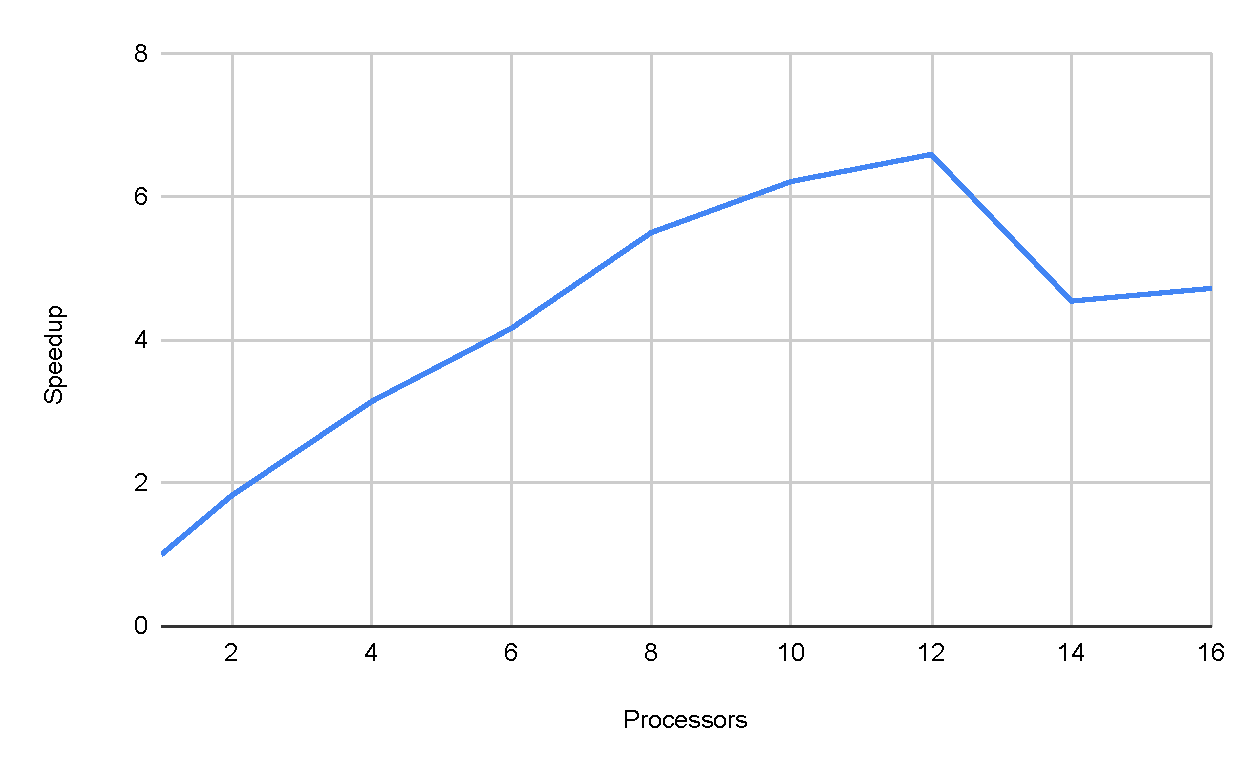
\includegraphics[scale=0.5]{strong}
\end{center}
\begin{itemize}
\item $A \in 3360\times3360$
\item 16-core machine
\end{itemize}
\end{frame}

\begin{frame}{Weak Scaling}
\begin{center}
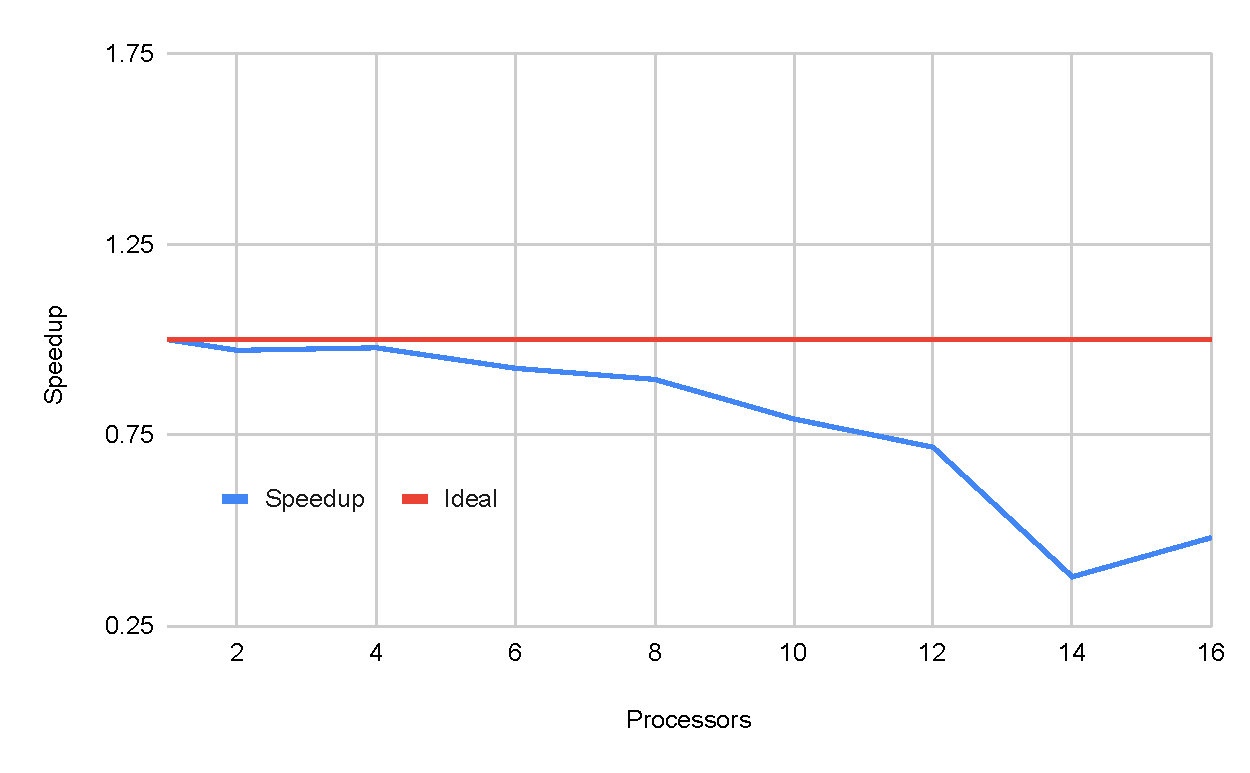
\includegraphics[scale=0.5]{weak}
\end{center}
\begin{itemize}
\item $\frac{mn}{p} = C$ so that each $p$ received the same size submatrix
\end{itemize}
\end{frame}

\begin{frame}{Future Work}
\begin{itemize}
\item Large-Scale scaling experiments (Cluster)
\item Document Clustering Algorithm using R2NMF
\end{itemize}
\end{frame}
\end{document}
